\documentclass[../main/main.tex]{subfiles}
\begin{document}
\chapter[Algorithms and implementation]{Algorithms and implementation}
In this chapter we focus our attention on specific integration algorithms. 
The first algorithm considered is the classic VEGAS algorithm \cite{Lepage:1977sw}. We discuss both techniques used in this thesis: importance sampling and stratified sampling. We also highlight its limitations.

Secondly we present in detail VEGAS+ \cite{Lepage:2020tgj}, a modification of the classic VEGAS algorithm which includes an adaptive stratified sampling technique.

After that we focus on a possible implementation of these algorithms based on hardware acceleration devices.
We analyze briefly an implementation of the VEGAS importance sampling algorithm using the TensorFlow library, \texttt{VegasFlow} \cite{Carrazza:2020rdn}, a MC integration library that enable us to run our computations on hardware acceleration devices such as GPUs. We highlight the role of TensorFlow as the back-end development framework and we discuss the most relevant achievements from Ref.~\cite{Carrazza:2020rdn}.

Finally, we present a novel implementation of the VEGAS+ algorithm within the \texttt{VegasFlow} library. 

 
	
\section{Algorithms}
During the last decade, several integration algorithms based on Monte Carlo methods have been proposed.
These algorithms usually implement the techniques of variance reduction presented in Section \ref{redu_var}: importance sampling and stratified sampling.

We will focus on two algorithms which employ both importance and stratified sampling: VEGAS and VEGAS+.

\subsection{VEGAS}
\label{vegas}
VEGAS is an algorithm for adaptive multi-dimensional MC integration formulated by Peter Lepage in 1977 in Ref.~\cite{Lepage:1977sw}.
Since then, it has been used in numerous fields including chemistry, applied finance and physics, among others.

VEGAS is widely used especially in HEP both as a MC event generator as well as to evaluate Feynman diagrams numerically.
In particular is the main driver for programs which perform QCD fixed-order calculations such as MCFM \cite{Campbell:2015qma, Campbell:2019dru}, NNLOJET \cite{Gehrmann:2018szu}. It also used for more general tools such as MG5\_aMC@NLO \cite{Alwall:2014hca} and Sherpa \cite{Gleisberg:2008ta}.
 
\subsubsection{Importance sampling}
VEGAS is primarily based on importance sampling but also features some stratified sampling techniques.
Using importance sampling, as we know from the previous chapter, the aim is to find a function $p$  that resembles the integrand $f$ which can easily be sampled. The sampling density implemented in the algorithm is a \emph{separable} multi-dimensional function:
\begin{equation}
	p \propto g(x_1,x_2,x_3,\dots,x_n) = g_1(x_1)g_2(x_2)g_3(x_3)\dots g_n(x_n) \ .
\end{equation}
The sampling of a $n$-dimensional vector $\textbf{x}=(x_1,x_2,x_3,\dots,x_n)$ is performed sampling the $n$-one dimensional sampling densities
$g_i$ to obtain the coordinates $x_i$ of the vector, which is far more simple than sampling a complex multi-dimensional function.

Moreover it can be shown \cite{Lepage:1977sw, Press:1989vk} that optimal weight functions are:
\begin{equation}
	\label{best VEGAS}
	 g_1(x_1) = \frac{\displaystyle \bigg[ \int dx_2 \dots \int dx_n \frac{f^2(x_1,\dots,x_n)}{g_2(x_2)\dots g_n(x_n) }\bigg]^\frac{1}{2}} { \displaystyle
	 	\int dx_1\bigg[ \int dx_2 \dots \int dx_n \frac{f^2(x_1,\dots,x_n)}{g_2(x_2)\dots g_n(x_n) }\bigg]^\frac{1}{2}} \ ,
\end{equation}
which suggests what will be VEGAS adaptive strategy: starting from a set of $g$-functions, when sampling the function $f$,  we can accumulate the
squared value of the function in each sampled point $\tilde{\textbf{x}}$, i.e.\ $f^2(\tilde{\textbf{x}})$  and then use this information 
to determine  the improved  $g_i$  functions iteratively based on Eq.~\ref{best VEGAS}.

The algorithm uses as sampling densities, step functions with a number of step $N$ fixed, that is divides each one-dimensional domain of integration which can be taken as $\interval{0}{1}$ \footnote{If the integral is defined between two generic integers $a$ and $b$ we can perform a change of variable with Jacobian $J(y)$ to simply change the boundaries from $\interval{a}{b}$ to $\interval{0}{1}$
\begin{equation}
	I = \int_a^b dx  f(x) = \int_0^1 dy J(y)f(x(y)) 
\end{equation}}
 in $N$ subintervals $\Delta x_i$ with the constraint:
\begin{equation}
	\sum_{i=1}^N \Delta x_i = 1 \ .
\end{equation}
The one-dimensional probability density of a random number being chosen from any given step $\Delta x_i$ is defined to be a constant equal to:
\begin{equation}
	g_i(x) = \frac{1}{N \Delta x_i} \ ,
\end{equation}
if $x$ is in the interval  $\{x_i - \Delta x_i, x_i \}$.

The probability distribution for each dimension is then modified in each iteration of the simulation by simply adjusting the increment sizes $\Delta x_i$.  It can be shown that the variance is minimized when the average value of $f^2(\textbf{x})$ in each interval is the same for every interval:

\begin{equation}
	\label{vegas importance optimal}
	\Delta x_i \int_{x_i - \Delta x_i}^{x_i} d\textbf{x} f^2(\textbf{x}) = \text{constant} \ .
\end{equation}
This approach is particularly effective for integrands with strong peaks since the algorithm will shorten the intervals where the function is peaked in order to achieve the optimal partition of intervals given by Eq.~\ref{vegas importance optimal}.

The variation of all the intervals $\Delta x_i$ is done iteratively. 
VEGAS initially estimates the integral with a uniform grid (all the intervals have the same length). Simultaneously, the algorithm  accumulates the quantities $d_i$ which are defined as:
\begin{equation}
	d_i \equiv \frac{1}{n_i} \sum_{x_j \in \interval{x_i - \Delta x_i}{x_i} } f^2(\textbf{x}) \approx \Delta x_i \int_{x_i - \Delta x_i}^{x_i} d\textbf{x} f^2(\textbf{x})  \ ,
\end{equation}
Using these parameters the algorithm presented in Ref.~\cite{Lepage:2020tgj} is able to generate new intervals $\{x'_i - \Delta x'_i, x'_i \}$ that contains an equal fraction of the total $d = \sum_i d_i$ thus fulfilling the constraint of Eq.~\ref{vegas importance optimal}.

To better understand the importance sampling used in VEGAS we show an example of an optimize grid.
Suppose that we need to compute the following integral:
\begin{equation}
	\label{example_integrand}
	\int_0^1 d^4 x \big(e^{-100(\textbf{x}- \textbf{r}_1)^2} + e^{-100(\textbf{x}- \textbf{r}_2)^2} \big) \ ,
\end{equation}
where $\textbf{x} = (x_1, x_2, x_3, x_4)$, $\textbf{r}_1 = (0.33, 0.5, 0.5, 0.5)$ and $\textbf{r}_2 = (0.67, 0.5, 0.5, 0.5)$.
\begin{figure}
	\centering
	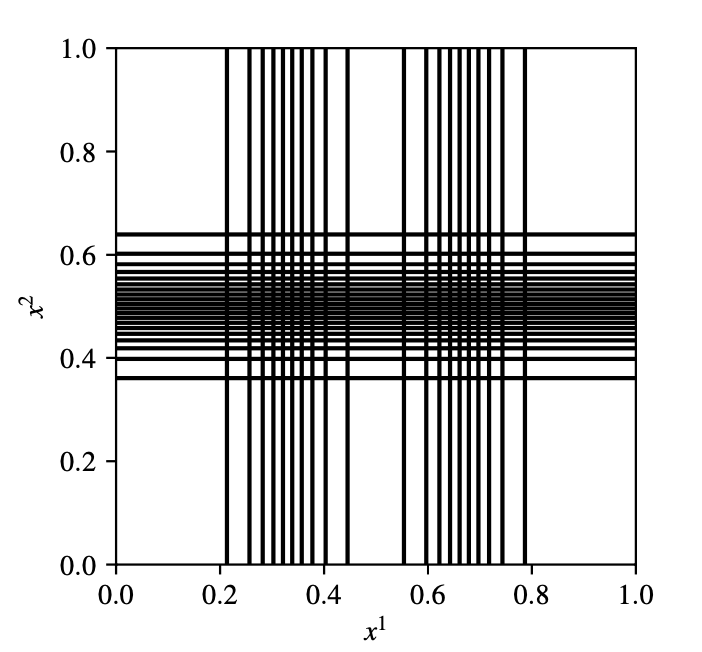
\includegraphics[width=8cm]{../images/vegas_grid.png}
	\caption{Vegas grid for the integral defined in Eq.~\ref{example_integrand}. Image from Ref.~\cite{Lepage:2020tgj}.}
	\label{vegas_grid}
\end{figure}
We expect that the optimized grid should shorten the intervals near $0.33$ and $0.67$ in the direction $x_1$ and near $0.5$ for all the 
other directions. This exactly what is shown in Fig.~\ref{vegas_grid}.

The importance sampling proposed in VEGAS is particularly effective for integrals like that one in Eq.~\ref{example_integrand} since the integrand function being a sum of Gaussians can be separated into a product of one-dimensional integrals over each direction.

The weakness of this algorithm is the obvious one: not all integrands can be approximated by their projections onto individual coordinate
directions. This is why VEGAS can struggle to converge with function whose geometry is non-separable or more in general if the integrand
is concentrated along one-dimensional (or higher) curved trajectories (or hypersurfaces) unless these happen to be aligned with the coordinate directions. The simplest case corresponds to a Gaussian peaked along a generic body diagonal line.


\subsubsection{Stratified Sampling}
VEGAS also employs standard stratified sampling techniques to reduce the variance.
Assuming to compute a $D$ dimensional integral each axis is divided into a fixed number of stratifications $N_\text{st}$, in particular using a total of $N_{\text{ev}}$ per iteration $N_\text{st}$ is computed as:

\begin{equation}
	\label{strat}
	N_\text{st} = \lfloor (N_\text{ev}/2)^{1/D}\rfloor \ ,
\end{equation}
which corresponds to dividing the $D$ dimensional volume into $N_\text{st}^D$ hypercubes of side $1/N_\text{st}$.

After that a MC integration is performed in each hypercube using $n_\text{ev}$ samples, the integral required $I$ can be computed as:
\begin{equation}
	\label{i str}
	I = \frac{V}{N_\text{st}^D}\sum_h \bigg(\frac{1}{n_\text{ev}} \sum_{\textbf{x} \in h} f(\textbf{x}) \bigg) = \sum_h I_h \ ,
\end{equation}
where $I_h$ denotes the integral estimate limited to hypercube $h$.

The variance can be computed using Eq.\eqref{var_stratified} as the sum of the variance in each hypercube:
\begin{equation}
	\label{sigma str}
	\sigma^2_I = \sum_h \sigma^2_h \ ,
\end{equation}
where $\sigma^2_h$ denotes the variance in the hypercube $h$.
In order to perform a MC integration in each hypercube we need to have at least $2$ integrand samples per hypercube. This requirement is already satisfied since the number of stratifications was defined in Eq.~\ref{strat} such that we will have at least 2 samples per hypercube. 

The algorithm uses the same number of samples per hypercube $n_\text{ev}$ defined as:
\begin{equation}
	n_\text{ev} = \lfloor (N_\text{ev}/N_\text{st}^D)\rfloor \ge 2 \ .
\end{equation} 
The addition to a stratified sampling techniques along side the importance sampling is surely useful.
However, as already discussed in Sect.~\ref{redu_var}, stratified sampling works better with low-dimensional integrals. For 
high-dimensional integrals huge samples are necessary to observe any considerable improvements.

\subsection{A new algorithm: VEGAS+}
\label{vegas+}
VEGAS, as we already discussed, struggles to converge with integrands that have non-trivial correlations between the integration variables. An integrand concentrated close to a body diagonal line, for example one from 
$(0,0,\dots,0)$ to $(1,1,\dots,1)$ shows a slower convergence since its geometry is completely non-separable. 
Also functions with multiple peaks can become challenging for the current implementation of VEGAS.

A new algorithm has been formulated which has been proven to perform better than classic VEGAS in these particular instances \cite{Lepage:2020tgj}.
This new method consists in a modification of the classic VEGAS by adding a second adaptive strategy in addition to the importance sampling, hence the name VEGAS+.

We saw that VEGAS also uses a stratified sampling by dividing the integration in $N_\text{st}^D$ hypercubes then performing a MC estimates of 
the integral using at least $2$ points per hypercube. In the classic implementation the number of samples per hypercube is the same for all the 
subvolumes.

VEGAS+ improves the stratified sampling techniques of VEGAS by allowing the number of integrand samples per hypercube to change from hypercube to hypercube. In particular these samples are redistributed iteratively in order to minimize the variance of the integral estimate using the 
samples of the previous iteration. We can therefore say that VEGAS+ employs an adaptive stratified sampling.

Moreover by allowing a redistribution of the samples this algorithm can include non-trivial correlations between the integration variables overcoming the separable-geometry approach of VEGAS.


The integral will be computed as before with the only difference that we need to define a new variable $n_h$ which represents the samples used 
in the hypercube $h$:

\begin{equation}
	I = \frac{V}{N_\text{st}^D}\sum_h \frac{1}{n_h} \sum_{\textbf{x} \in h} f(\textbf{x})  = \sum_h I_h \ .
\end{equation}

Now the expression for the variance in Eq.~\ref{sigma str} must be modified to include the different number of samples:
\begin{equation}
		\sigma^2_I = \sum_h  \frac{\sigma^2_h}{n_h} \ .
\end{equation}
Let us show briefly that the variance is minimized when the number of samples $n_h$ is proportional to the standard deviation of the hypercube 
$\sigma_h$.
The samples per hypercube $n_h$ are subject to the constraint that the sum of the points sampled in each hypercube  must be equal to the total number of sampled
points $N_\text{ev}$:
\begin{equation}
	N_\text{ev} = \sum_h n_h \ .
\end{equation}
We can find the optimal $n_h$ subject to the previous constraint using the method of Lagrange multipliers:
\begin{equation}
	0 = \frac{\delta}{\delta n_h} \bigg( \sum_k \frac{\sigma^2_k}{n_k} + \lambda \sum_k n_k\bigg) =  - \frac{\sigma^2_h}{n^2_h} + \lambda \ .
\end{equation}
Being $\lambda$ constant we get that the previous equation is satisfied if
\begin{equation}
	n_h \propto \sigma_h \ .
\end{equation}

The algorithm presented in Ref.~\cite{Lepage:2020tgj} redistribute the samples in the hypercubes as follows:

\begin{enumerate}
	\item Choose as number of stratifications
	\begin{equation}
		\label{nstrat}
		N_\text{st} = \lfloor (N_\text{ev}/4)^{1/D}\rfloor  \ .
	\end{equation}
\item 
During each iteration estimate the variance of each hypercube with same samples used to compute the integral
\begin{equation}
	\sigma^2_h \approx \frac{V_h^2}{n_h} \sum_{\textbf{x} \in V_h} f^2(\textbf{x}) - \bigg( \frac{V_h}{n_h} \sum_{\textbf{x} \in V_h} f(\textbf{x})\bigg)^2 \ ,
\end{equation}
where $V_h$ is the hypercube volume
\item Replace the variance by introducing a damping parameter $\beta \ge 0$ as:
\begin{equation}
	d_h \equiv \sigma_h^\beta \ ,
\end{equation}
with default value $\beta = 0.75$
\item 
Recalculate the number of samples for each hypercube to use in the next iteration:
\begin{equation}
	n_h = \text{max} \big(2, d_h / \sum_{h'} d_{h'}\big) \ .
\end{equation}
\end{enumerate}
Let us now comment briefly the algorithm.

Firstly, we can observe that the number of stratifications chosen is smaller than the one used in VEGAS (Eq.~\ref{strat}). This is done in order to
have enough samples in each hypercube to have a better estimates of the variance and more significant variations for the $n_h$. 

Secondly, the damping parameter $\beta$ is being introduced to avoid overreactions to random fluctuations in the first steps of the simulation. The optimal choice will be $\beta=1$, in the limit where $\beta=0$ we have VEGAS usual stratified sampling without the redistribution of samples.

At the same time after each iteration the VEGAS map is updated according to the standard VEGAS importance sampling algorithm. The optimal VEGAS grid is independent of the allocation of samples, but the reallocation of samples can speed the convergence to the optimal map. This is due to the fact that by reallocating the samples we are able to find more quickly all the peaks of the integrand, even for diagonal structures.
In fact Ref.~\cite{Lepage:2020tgj}considered the following diagonal-structured integral:
\begin{equation}
	\label{example_vegas+}
	\int_0^1 d^8 x \sum_{i=1}^3 e^{-50 |\textbf{x}- \textbf{r}_i|}
\end{equation}
where the peaks are distributed along the diagonal:
\begin{eqnarray*}
	\textbf{r}_1 &= (0.23,0.23,0.23,0.23,0.23,0.23,0.23,0.23)  \\
	\textbf{r}_2 &= (0.39,0.39,0.39,0.39,0.39,0.39,0.39,0.39)  \\
	\textbf{r}_3 &=(0.74,0.74,0.74,0.74,0.74,0.74,0.74,0.74)  
\end{eqnarray*}
Fig.~\ref{vegas_vegas+} shows the speed of convergence of classic VEGAS and VEGAS+ for the previous integral. We can see that classic VEGAS becomes unstable below $N_\text{ev} =3 \times 10^6$ while VEGAS+ is unstable below $N_\text{ev} =1 \times 10^5$. Moreover
VEGAS+ is overall the most accurate integrator for this particular integral.

\begin{figure}[h]
	\centering
	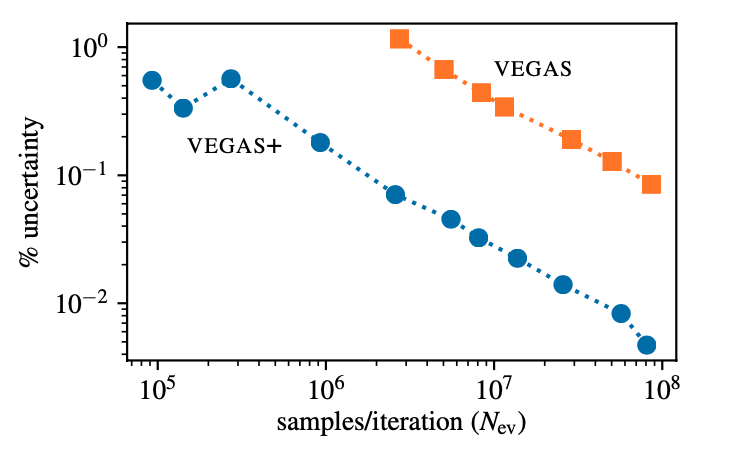
\includegraphics[width=10cm]{../images/VEGAS-VEGAS+.png}
	\caption{Image from Ref.~\cite{Lepage:2020tgj} showing the percent uncertainty in the integral estimates of Eq.~\ref{example_vegas+} from 30 iterations of classic VEGAS, which uses importance sampling and stratified sampling,  and VEGAS+.}
	\label{vegas_vegas+}
\end{figure}

\subsubsection{Limitations}
The adaptive stratified sampling suffers from the same limitations of the standard adaptive stratified sampling.
We need a larger number of samples compared to the importance sampling  to have significant effects for high-dimensional integral.
From Eq.~\ref{nstrat} we can observe that the number of stratifications $N_\text{st}$ grows with the number of events as 
\begin{equation}
	N_\text{st} \approx N_\text{ev}^{1/D} \ ,
\end{equation}
therefore the number of stratifications is suppressed as the dimension increases. 

\section{Implementation}
In this section we discuss a novel implementation of the algorithms aforementioned.
In particular the VEGAS algorithm has been available since the '80s and has been implemented in different programming languages.
The new VEGAS+ algorithm is currently available at Ref.~\cite{peter_lepage_2021_4746454}.
The original implementations are usually written for a single CPU or at most they support multi-processor evaluation of integrands using
MPI, via the python module \texttt{mpi4py} \cite{peter_lepage_2021_4746454}.

We have instead decided to focus on an implementation that can also run in hardware acceleration devices such as multi-threading CPUs and GPUs.

\subsection{VegasFlow: a brief overview}
\texttt{VegasFlow} \cite{vegasflow_package} is the first implementation of the VEGAS algorithm that is able to run both on CPUs and GPUs.
 
The aim of the library is to exploit the paralelizability of MC computations thus lowering the long CPU-times usually required especially when
dealing with HEP integrands.
 \texttt{VegasFlow} achieves this goal using the TensorFlow library \cite{tensorflow2015-whitepaper}, which is primarily used for deep learning applications, as the back-end development framework. 

\subsubsection{Why TensorFlow?}
\label{tensorflow}

TensorFlow (TF) has a simple mechanism that enable us to write python code which can be distributed to hardware 
 acceleration devices without complicated installation procedures.
 
 In particular there is no need to write a different version of the code whether we run it on CPU or GPU. Once TF has found different devices, for example a CPU and a GPU, we can choose where to run a specific set of instructions by using the primitive \texttt{tf.device}.
 By default TF will run on GPU if available.
 
\begin{minted}[fontsize=\footnotesize]{python}
import tensorflow as tf

with tf.device('/CPU:0'):
	# these operations will run on CPU
	a = tf.constant([[1.0, 2.0, 3.0], [4.0, 5.0, 6.0]])
	b = tf.constant([[1.0, 2.0], [3.0, 4.0], [5.0, 6.0]])
		
# this will run on GPU	
c = tf.matmul(a, b)
\end{minted}

Secondly, TF has two execution modes one is the so called eager mode and the other one uses graphs to compile the operations written in python.

The eager execution, which is turned on by default, implements an imperative programming environment that evaluates operations immediately: each operation returns concrete values. 

There is also the possibility to create and run a  TF graph by adding the decorator \texttt{@tf.function} to the functions defined by the user. In particular the function defined with such decorator will be a python callable that builds TensorFlow graphs from the python function.
A TF graph requires that his input must have a specified data and dimension type since it cannot contains all the statements of the eager program. The code is separated in two stages:
\begin{enumerate}
	\item In the first step a graph is created by the function, all the python code runs normally while the statement expressed by TF primitives are deferred: they are simply stored in the graph. This first step is referred as \emph{tracing}.
	\item In the second step the graph created in the first one is run.
\end{enumerate}

One of the main advantages is that the second step is much faster than the first one, due to the fact that the statements have been converted to a graph. 
Graphs are easily optimized and allow the compiler to do transformations like separating sub-parts of a computation that are independent and splitting them between threads or devices.
If a function is called more than once with the same arguments the first step, the \emph{tracing}, will be performed only the first time. In all the successive calls of the function the first step will be skipped since TF already as a graph available for that particular function.
This possibility of skipping the tracing step is what enable TF to reach better performances when compared to the eager mode. 

This feature can be exploited in MC simulation where we expect to call a function a different number of times depending on the accuracy required. 

\subsubsection{Design and algorithms}
The library has an abstract class called \texttt{MonteCarloFlow} which implements the distribution
of events across multiple devices with a job scheduling for multi-GPU synchronization using TF graph technology.

The proper MC integrators are implemented as derived class from the \texttt{MonteCarloFlow} class. The library provides two different integrators: one is a vey simple MC integrator in the class \texttt{PlainFlow} and the main one is an implementation of Vegas's importance sampling algorithm in the class \texttt{VegasFlow}.
The ladder one is the first implementation of the importance sampling algorithm in VEGAS using TensorFlow as the back-end development framework.
The two subclasses focus only on the integration algorithm chosen, in particular they need to specifies what the algorithm does to run one single event and secondly what to do in a full iteration of the MC simulation.

Therefore the library is designed such that new algorithms can easily be implemented as derived class from the \texttt{MonteCarloFlow} abstract class which handles all the technicalities such as GPU distribution, multi-threading or vectorization.
The developer, as already shown in the integrators available, should only focus on what the integrators do for a single event and in a full iteration.

 
 \subsubsection{Results}
We now comment some results of \texttt{VegasFlow} presented in Ref\cite{Carrazza:2020rdn}.
\texttt{VegasFlow} (running on both CPU and GPU) has been compare to the current implementation of the Vegas importance sampling algorithm available in python \cite{peter_lepage_2021_4746454}. The results show that in order to reach the same accuracy integrating a Gaussian distribution in 20 dimension the previous implementation of VEGAS takes  38 minutes, while VegasFlow running on CPU\footnote{\setstretch{1}These results are obtained using all CPUs (36 threads) from an Intel(R) Core(TM) i9-9980XE CPU for both Vegas and \texttt{VegasFlow}.} takes 26 minutes and only 5 minutes when running of GPU \footnote{The GPU used is the NVIDIA Titan V.}.
Therefore as expected when \texttt{VegasFlow} runs on GPU there are some significant improvements in the computational times.

Moreover, \texttt{VegasFlow} shows better performance thanks to the graph compilation mode when running on highly parallel scenarios such as
multi-CPU computation or GPU as shown in Fig.~\ref{vegasflow1}

\begin{figure}
	\centering
	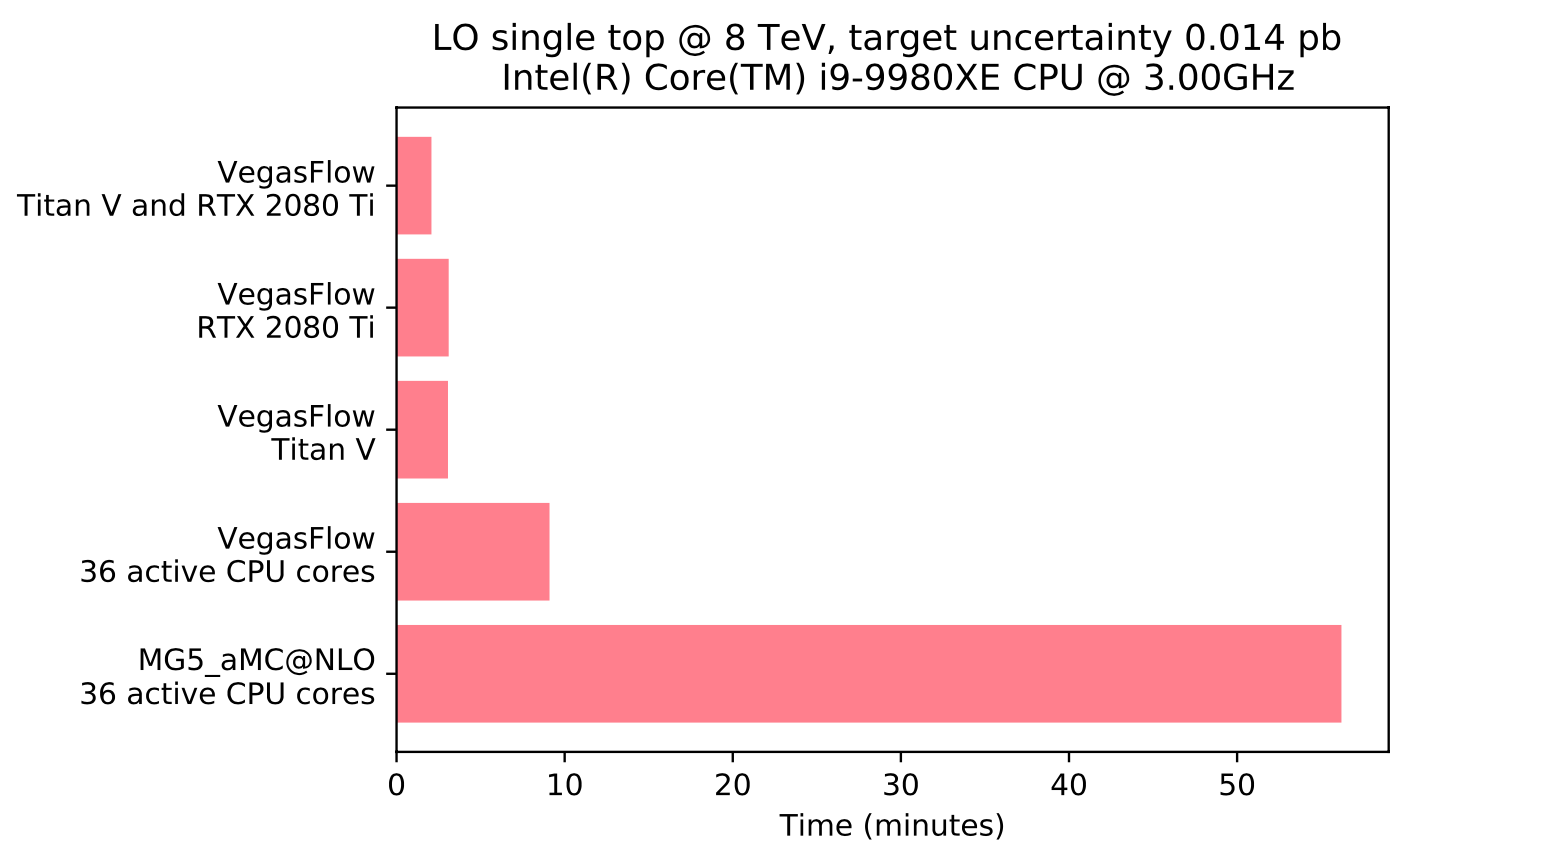
\includegraphics[width=12cm]{../images/graph_mode.png}
	\caption{Comparison of performance between the eager and graph compilation TensorFlow mode. The results are shown as a ratio of the time it took the eager computation to complete one iteration. Image from Ref.~\cite{Carrazza:2020rdn}.}
	\label{vegasflow1}
\end{figure}


Finally, \texttt{VegasFlow} has been confronted with MadGraph5\_aMC@NLO \cite{Alwall:2014hca} for the computation of the single $t$-quark production at the partonic level at leading order. The results in Fig.~\ref{vegasflow2} show how \texttt{VegasFlow} can outperform  MadGraph5\_aMC@NLO while running on CPU and even more on GPU.

\begin{figure}
	\centering
	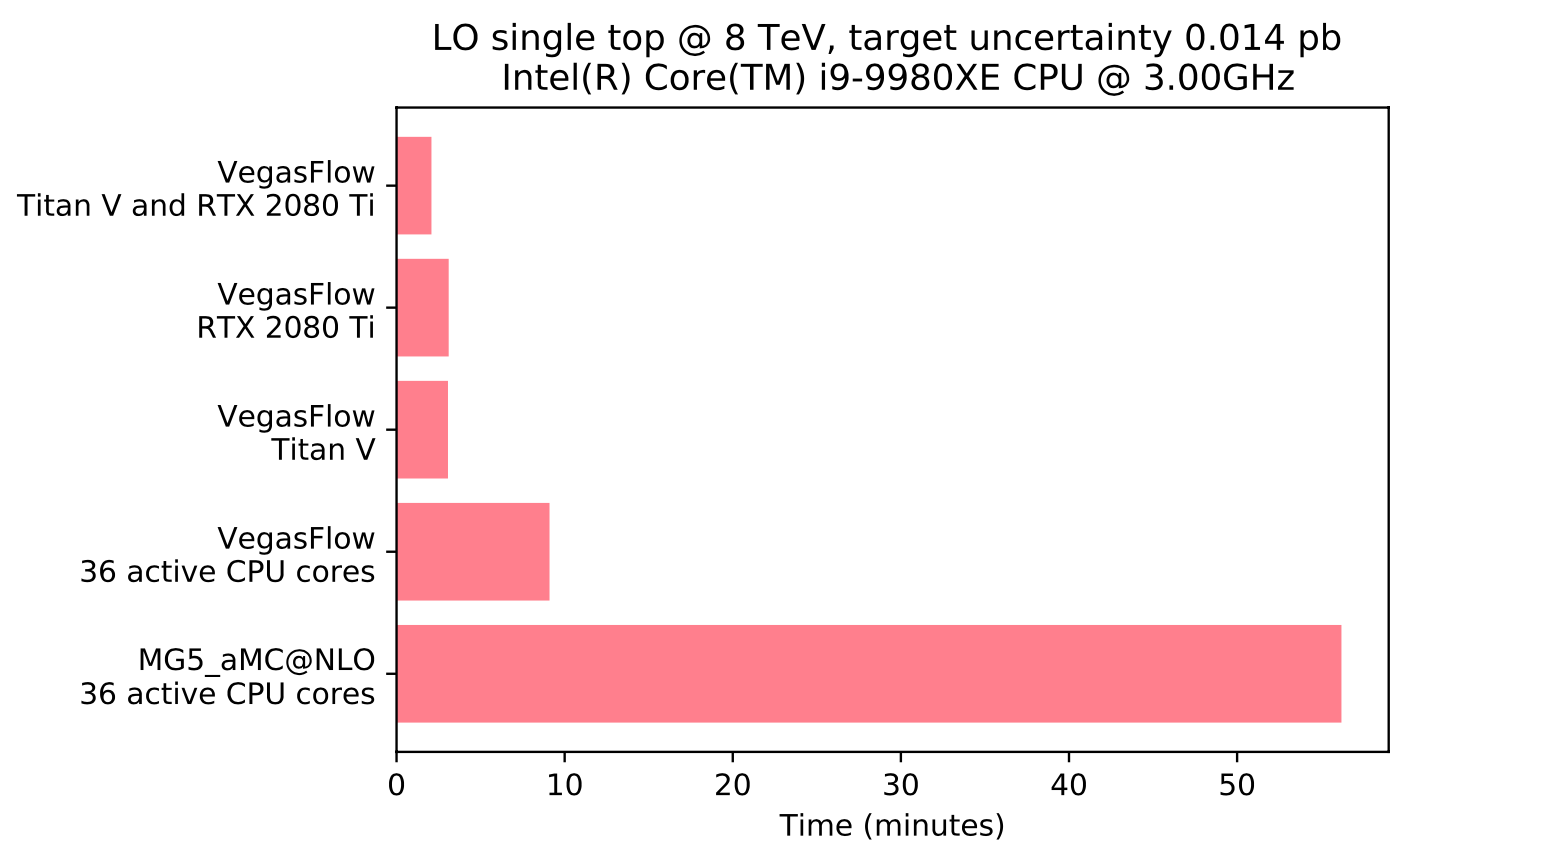
\includegraphics[width=12cm]{../images/vf_singletop.png}
	\caption{Comparison of a Leading Order calculation ran in both \texttt{VegasFlow} \cite{vegasflow_package} and MG5\_aMC@NLO \cite{Alwall:2014hca}. For the same level 
	of target accuracy \texttt{VegasFlow} is faster than  MG5\_aMC@NLO when using both CPUs and GPUs devices. Image from Ref.~\cite{Carrazza:2020rdn}.}
	\label{vegasflow2}
\end{figure}

 
 
 
 
\subsection{A new implementation: VegasFlowPlus}
In this thesis we present a novel implementation of the VEGAS+ algorithm within the framework of the \texttt{VegasFlow} library.
\subsubsection{Motivation}
As we already observed in the \texttt{VegasFlow} library the primarily algorithm is the VEGAS importance sampling algorithm, which has been proven to be effective for multi-dimensional integration.

\texttt{VegasFlow} has shown remarkable performances compared with the importance sampling  implemented in python \cite{peter_lepage_2021_4746454} thanks to the support of hardware acceleration devices . Obviously in order to reach the same accuracy level the number of iterations was roughly the same since the two integrators are based on the same algorithm.

In order to reach better performances we consider the possibility of implementing more accurate algorithms in the \texttt{VegasFlow} library, i.e.\ integrators that converge using less events per iteration or less iterations. 

In particular we have considered the VEGAS+ algorithm as a possible candidate. 
As we already discussed in Sect.~\ref{vegas+} VEGAS+ employs a new technique called adaptive stratified sampling together with the importance sampling algorithm. 
We benchmarked the performances of the importance sampling compared to the new VEGAS+ algorithm and the adaptive stratified sampling technique alone to see whether one of them can outperform the importance sampling method.

The benchmark was performed using the python implementation of the VEGAS algorithm \cite{peter_lepage_2021_4746454}.
We first performed a dimensional comparison, i.e.\ we tested the three methods with integrands of different dimensions to see which integrators shows better accuracy the results are shown in Fig.~\ref{gauss_dim} and Fig.~\ref{rosen_dims}.


We can observe that VEGAS+ seems to be the more accurate integrator in general. Moreover, we can see that for the Gaussian distribution the adaptive stratified sampling is by far the less precise integrator due to the sharp peak of the distribution. For the case of the RosenBrock \cite{10.1093/comjnl/3.3.175} function  we can see that the adaptive stratified sampling can outperform the importance sampling only for dimension less than 5. This is expected since the stratified sampling struggles to converge in higher dimensions.

\begin{figure}[h]
	\centering
	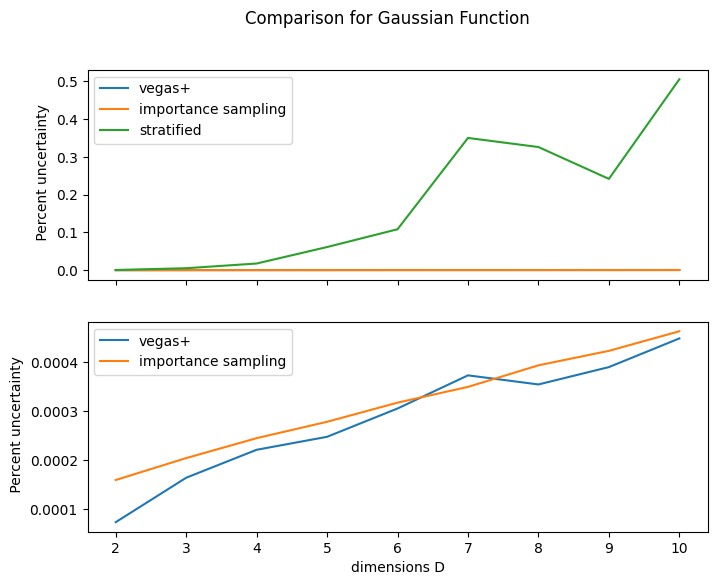
\includegraphics[width=10cm]{../../../tests/plots/gauss_dims_2.png}
	\caption{Comparison of  percent uncertainty of Gaussian integral  from 50 iterations with 12000 samples after a warmup of 5 iterations with 1000 samples. }
	\label{gauss_dim}
\end{figure}

\begin{figure}[h]
	\centering
	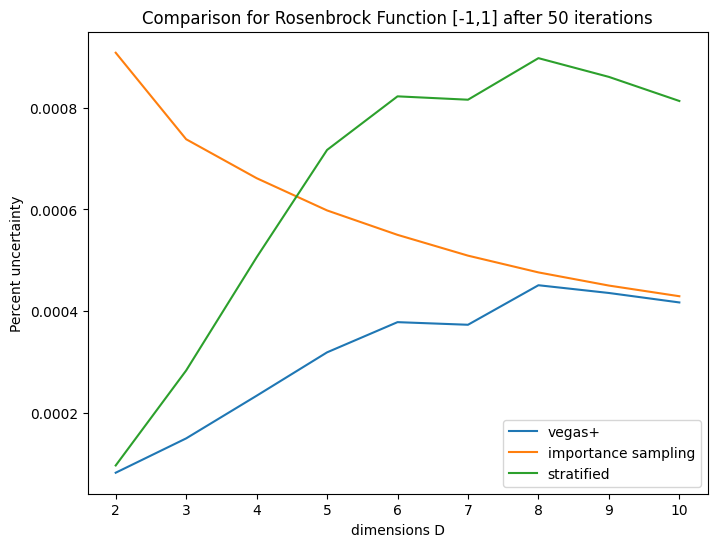
\includegraphics[width=10cm]{../../../tests/plots/rosen_dims_final.png}
	\caption{Comparison of  percent uncertainty of Gaussian integral  from 50 iterations with 12000 samples after a warmup of 5 iterations with 1000 samples. }
	\label{rosen_dims}
\end{figure}


We also performed a comparison based on the number of samples which showed that in general using the same number of samples VEGAS+
converged more rapidly than the importance sampling. The adaptive stratified sampling converged more slowly and only with a large number of samples can sometimes reach the accuracy of the other two methods.

Finally, we have also considered a performance comparison, i.e.\ at fixed samples per iteration we have considered the number of iterations needed in order to reach the accuracy required.
The most relevant result was obtained using a physical integrand, the Leading Order (LO) partonic cross section for the Drell-Yan process from Ref.~\cite{Carrazza_2020}.
We noted that VEGAS+ was the integrator that performed better and was the only one that achieved a percent uncertainty of 0.0001 \% within a maximum of 100 iterations.
The possibility of reaching the target accuracy using less than 20 iterations leads to significant improvements also in the computational time. 

\begin{figure}
	\centering
	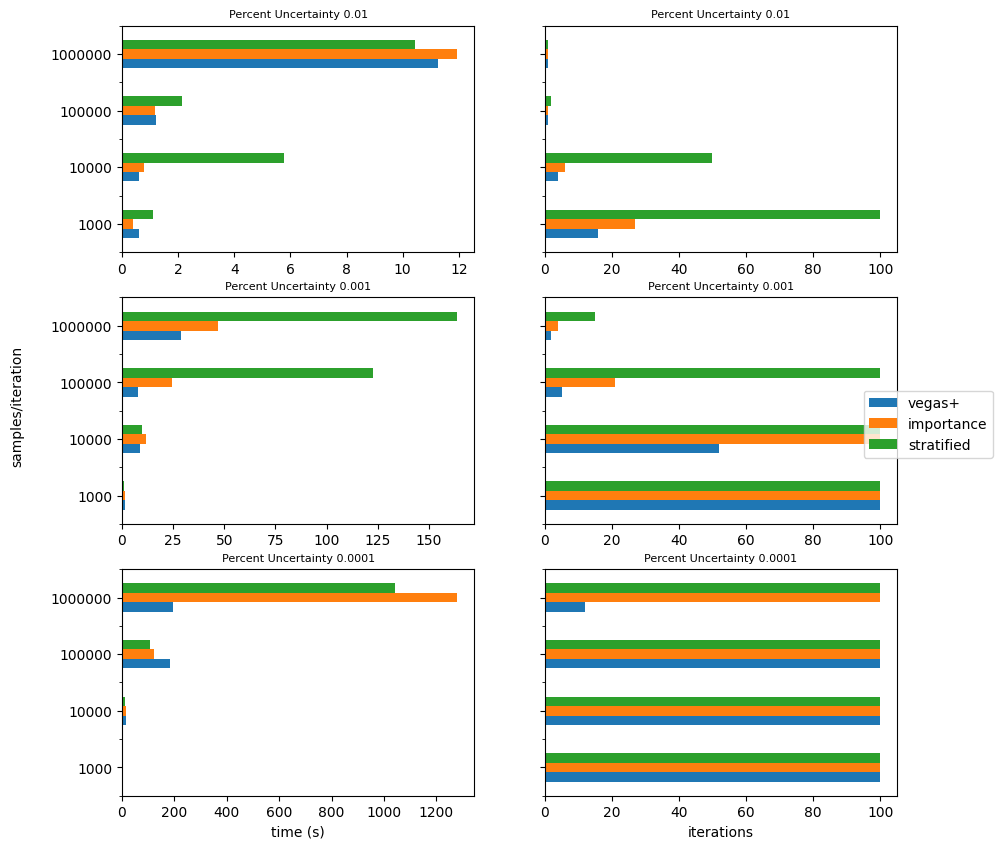
\includegraphics[width=15cm]{../../../tests/performance_plots/dy_aa.png}
	\caption{Comparison of perfomances between different integration methods at fixed percent uncertainty ( $10^{-2}$, $10^{-3}$ or $10^{-4}$) and at fixed samples per iteration ($10^3$,$10^4$,$10^5$ or $10^6$ ) with $100$ maximum iterations. The integrand used is the LO partonic cross section for the Drell-Yan process from Ref.~\cite{Carrazza_2020}.}
	\label{dy_aa}
\end{figure}

Overall all the tests performed show that VEGAS+ is  the more efficient integration algorithm and can outperform the implementation of the importance sampling in VEGAS. The adaptive stratified sampling alone was effective only with low-dimensional integrands without sharp peaks, like the RosenBrock function. In general, it couldn't compete with the other two methods.

Moreover, the fact that for a physical integrand VEGAS+ converged way more rapidly than the importance sampling convinced us even more to exploit the VEGAS+ algorithm by running it on hardware acceleration devices.


\subsubsection{Implementation}
To implement the VEGAS+ algorithm within the \texttt{VegasFlow} library we exploit the possibility of adding new algorithms simply by
adding classes derived from the \texttt{MonteCarloFlow} class. Moreover, since the VEGAS+ algorithm contains the same importance sampling method already implemented in the \texttt{VegasFlow} class we decided to create a derived class from the \texttt{VegasFlow} class called \texttt{VegasFlowPlus}

The next step was to implement all the machinery of the stratified sampling. 
One of the main difference is the process of sampling. Using only importance sampling the points are sampled from all the integration domain accordingly to the sampling distribution which is a grid refined in every iterations. Using stratified sampling instead, we need to divide the integration domain in a certain number of hypercubes and we need to extract a specific number of points from each hypercube. 
Thus, we introduced a new function \texttt{generate\_samples\_in\_hypercubes} that implements this different type of sampling.

Moreover, since we are interested in the VEGAS+ algorithm, in which the points sampled are no longer fixed in every hypercube but change accordingly to the variance in each one, we have also introduced a tensor \texttt{n\_ev} which contains the number of samples in each hypercube. 
After each iteration this tensor is updated according to the VEGAS+ algorithm explain in section \ref{vegas+} by the method \texttt{redistribute\_samples} that receives as input a tensor containing the variance computed in each hypercube.

Finally, we also needed to overload the fundamental methods of the class that describe what the integrator should do for each event and for each iteration of the simulation. In particular since the integral is expressed as a contribution from a MC estimate of the integral in each hypercube both the integral estimate and the variance are computed by summing the partial results from all the hypercubes according to Eq.~\ref{i str} and Eq.~\ref{sigma str}.

All the implementation is publicly available at the following GitHub repository: \url{https://github.com/N3PDF/vegasflow}.
\subsubsection{Problems during the implementation}
\label{vfp problem}
The process of implementing the VEGAS+ algorithm within the \texttt{VegasFlow} library has not been free of problems.

The choice of TensorFlow was motivated also by the fact that the graph implementation enable us to achieve better performances. In particular if a function is called more than once the program will refer to the same graph of the function if the type and the shape of the input tensors are the same.
Both the importance sampling and the stratified sampling can benefits from this since all the tensors don't change size from one iteration to another. However the new feature of VEGAS+, i.e., the adaptive stratified sampling does not maintain the same shape for all the tensors.
In fact when calling the method \texttt{redistribute\_samples} the total number of events used in each iterations changes since the algorithm does not maintain exactly the same number of samples.
Therefore when executing the program we will not be able to skip the tracing step, but for every iteration of the simulation we will  need to generate new graphs for all the functions that involve the total events per iteration. This problem is known as \emph{retracing} and leads to worst performances especially if the function that causes the retracing is called a large of number of times.

The TensorFlow library offers a way around the \emph{retracing} problem.
In particular one can specify a \texttt{input\_signature} in a function defined with the decorator \texttt{@tf.function}.
Through the \texttt{input\_singnature} we can specify both the type and the shape of the input tensors, by setting one or more dimensions to \texttt{None} in the shape we can allow for flexibility in the trace reuse. Below we can see an example of the use of the \texttt{input\_singnature} from the source code of the \texttt{VegasFlowPlus} class.
\begin{minted}[fontsize=\footnotesize]{python}
@tf.function(input_signature=3 * [tf.TensorSpec(shape=[None, None], dtype=DTYPE)])
def _compute_x(x_ini, xn, xdelta):
	""" Helper function for generate_samples_in_hypercubes """
	aux_rand = xn - tf.math.floor(xn)
	return x_ini + xdelta * aux_rand
	
\end{minted}
Therefore we made all the programming environment flexible with respect to the number of events used in each iteration by specifying an input signature for each function.

There was a second problem the VEGAS+ algorithm.
We experienced some crashes while the program was running due to a high CPU usage even for high performing machines. After some tests we found out that when generating the samples per hypercube there was a problem with the primitive of TensorFlow \texttt{tf.repeat}. In particular inside the function at some point a rank-3 tensor was initialized using the total number of hypercubes, the dimension of the integrand and the maximum number of samples in one hypercube. Due to some overreaction of the algorithm in the first iterations the redistribution of the samples can accumulate a large number of samples in one particular hypercube. This lead to rank-3 tensors such as \texttt{[65536,51749,8]} which are too big to handle even for professional-grade CPUs and GPUs.

To solve this issue we decided to modify the program in the following way.
First of all we tried to reach the same output desired using alternatives to \texttt{tf.repeat}. These options could lower the CPU-usage however there were still some problems involving \texttt{tf.repeat}. So we decided to simply put a limit of $10000$ maximum hypercubes because by limiting the number of hypercubes we could avoid the big tensors that caused the problems.
Moreover,  we decided to turn off the adaptive stratified sampling for high-dimensional integrands ($D > 13$) since it cannot be effective unless we use a bigger number of hypercubes.

\end{document}